\chapter{Kunststoffen en synthetische materialen}\label{ch:g8:plastics}

Tel de plastic voorwerpen die je op één ochtend aanraakt: een
tandenborstel, een fles, een regenjas, een telefoonhoesje, de stoel in de
bus, de boodschappentas. Bijna geen ervan bestond honderdtwintig jaar
geleden, en geen enkel ervan groeide aan een boom of werd uit de grond
gegraven. \omterm{def:g8:plastics:plastic}{Kunststoffen} zijn materialen die scheikundigen hebben
uitgevonden --- licht, goedkoop, waterdicht, in elke vorm te brengen ---
en juist dat succes is een probleem geworden.

\begin{recall}
\omterm{def:g5:raw-materials-and-recycling:natural-material}{Natuurlijke materialen} gebruik je ongeveer zoals je ze in de natuur
vindt; \omterm{def:g5:raw-materials-and-recycling:natural-material}{vervaardigde materialen} worden van \omterm{def:g5:raw-materials-and-recycling:raw-material}{grondstoffen} gemaakt door die
te veranderen, en \omterm{def:g5:raw-materials-and-recycling:recycling}{recycling} maakt van het materiaal van oude voorwerpen
nieuwe voorwerpen (\cref{ch:g5:raw-materials-and-recycling}). De
\omterm{def:g4:what-a-fire-needs:burning}{verbranding} van een \omterm{def:g4:what-a-fire-needs:fuel}{brandstof} uit koolstof en waterstof geeft
koolstofdioxide en water (\cref{ch:g8:combustion-and-fuels}).
\end{recall}

\begin{omfigure}
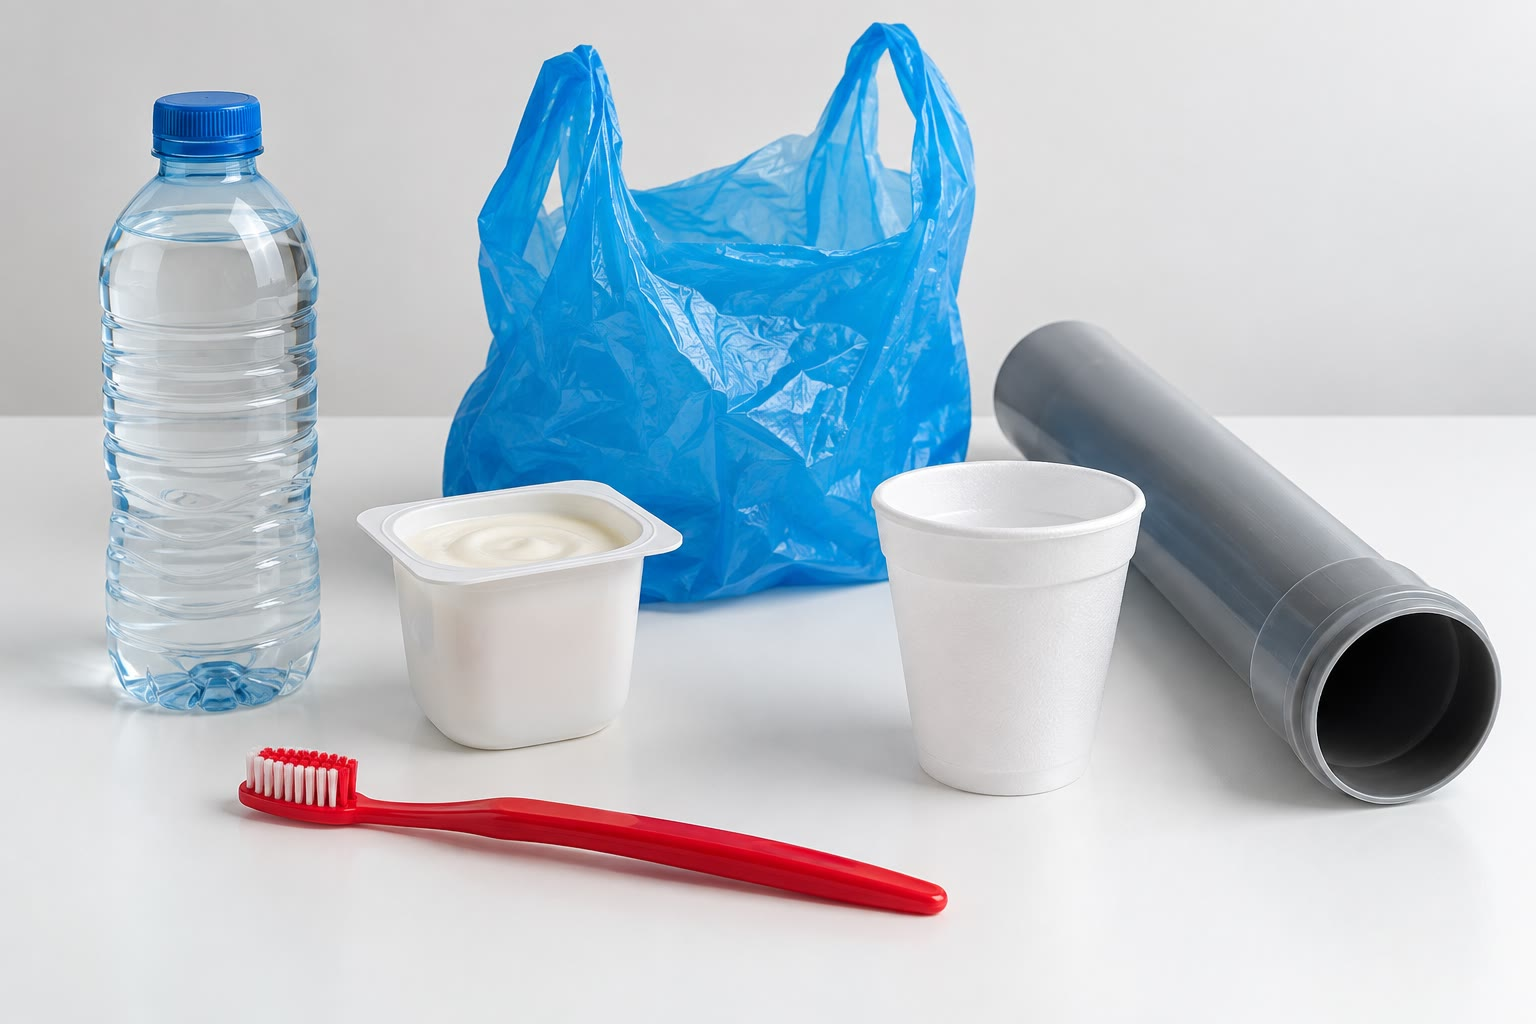
\includegraphics[width=0.55\linewidth]{images/book1/ai/g8-plastic-objects.jpg}

{\small Alledaagse plastic voorwerpen: een fles, een bakje, een tas, een
buis, een beker, een tandenborstel.}
\end{omfigure}

\section{Natuurlijke, kunstmatige en synthetische materialen}

\begin{definition}[Kunstmatige en synthetische materialen]\label{def:g8:plastics:artificial}
Onder de \omterm{def:g5:raw-materials-and-recycling:natural-material}{vervaardigde materialen} is een \emph{kunstmatig
materiaal}\index{kunstmatig materiaal} gemaakt door een \omterm{def:g5:raw-materials-and-recycling:natural-material}{natuurlijk
materiaal} chemisch om te zetten: papier en viscose (een textiel) uit de
cellulose van hout. Een \emph{synthetisch materiaal}\index{synthetisch materiaal}
wordt gemaakt uit stoffen die scheikundigen hebben opgebouwd, meestal
uit aardolie, en heeft geen tegenhanger in de natuur: nylon, polyester,
de \omterm{def:g8:plastics:plastic}{kunststoffen}.
\end{definition}

\begin{omfigure}
\begin{tikzpicture}[font=\small, level distance=1.5cm,
    box/.style={draw=omDef, fill=omDef!6, rounded corners=2pt, align=center,
      inner sep=4pt, text width=3.3cm},
    level 1/.style={sibling distance=6.4cm},
    level 2/.style={sibling distance=3.8cm},
    edge from parent/.style={draw, thick, omDef, ->}]
  \node[box] {materialen}
    child {node[box] {natuurlijk\\ \footnotesize katoen, wol, hout}}
    child {node[box] {vervaardigd}
      child {node[box] {kunstmatig\\ \footnotesize papier, viscose}}
      child {node[box, draw=omProp, fill=omProp!6] {synthetisch\\ \footnotesize nylon,
        polyester, kunststoffen}}};
\end{tikzpicture}

{\small Natuurlijke, kunstmatige en \omterm{def:g8:plastics:artificial}{synthetische materialen}.}
\end{omfigure}

\section{Wat kunststoffen zijn}

\begin{definition}[Kunststof]\label{def:g8:plastics:plastic}
Een \emph{kunststof}\index{kunststof} (in de omgangstaal: plastic) is
een \omterm{def:g8:plastics:artificial}{synthetisch materiaal} uit zeer lange \omterm{def:g7:atoms-and-molecules:molecule}{moleculen}, dat je kunt vormen
door het in een mal te gieten of te persen --- meestal terwijl het heet
en zacht is --- en dat zijn vorm houdt als het afkoelt. De meeste
kunststoffen worden gemaakt van aardolie of aardgas.
\end{definition}

\begin{remark}[Zeer lange moleculen]\label{rem:g8:plastics:long}
Een watermolecuul bevat drie \omterm{def:g7:atoms-and-molecules:atom}{atomen}; een \omterm{def:g7:atoms-and-molecules:molecule}{molecuul} van een \omterm{def:g8:plastics:plastic}{kunststof} kan
er tienduizenden bevatten, verbonden in een lange keten, zoals een
ketting van gelijke kralen. Hoe zulke ketens worden opgebouwd, is het
onderwerp van een hoofdstuk aan het eind van dit boek.
\end{remark}

\begin{omfigure}
\begin{tikzpicture}[font=\small]
  \foreach \k in {0,...,17} {
    \pgfmathsetmacro\x{0.62*\k}
    \pgfmathsetmacro\y{0.35*sin(40*\k)}
    \shade[ball color=omDef!50] (\x,\y) circle (0.22);
  }
  \node[anchor=west] at (11.2,0) {\dots};
  \node[anchor=north, align=center] at (5.3,-0.6) {een keten van duizenden gelijke eenheden};
\end{tikzpicture}

{\small Een plaatje, geen model: het \omterm{def:g7:atoms-and-molecules:molecule}{molecuul} van een \omterm{def:g8:plastics:plastic}{kunststof} is een
zeer lange keten van gelijke eenheden.}
\end{omfigure}

\begin{history}[Bakeliet, 1907]
De eerste volledig synthetische \omterm{def:g8:plastics:plastic}{kunststof} werd in 1907 gemaakt door de
scheikundige Leo Baekeland, uit fenol, gewonnen uit koolteer, en
formaldehyde. Bakeliet, hard, donker en hittebestendig, werd het
materiaal van telefoons, radio's en lichtschakelaars. In de jaren 1930
volgde nylon, en na de Tweede Wereldoorlog de \omterm{def:g8:plastics:plastic}{kunststoffen} van flessen en
tassen.
\end{history}

\begin{omfigure}
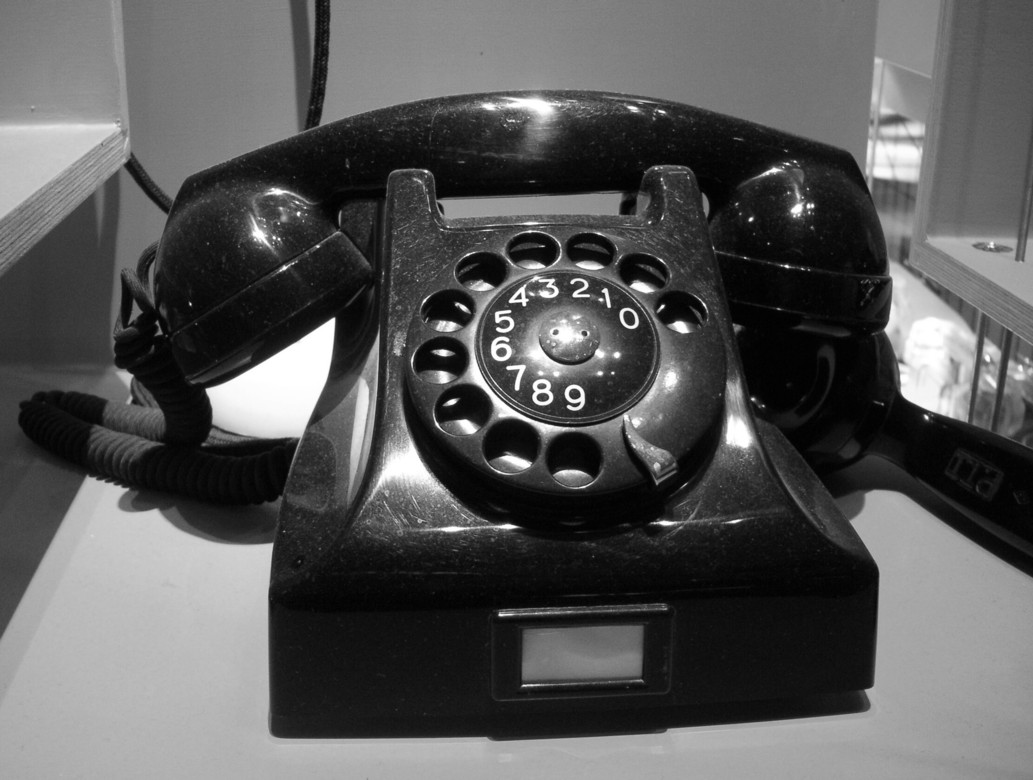
\includegraphics[width=0.42\linewidth]{images/book1/bakelite-telephone.jpg}

{\small Een bakelieten telefoon uit 1947. Foto: Holger Ellgaard,
CC BY-SA 3.0.}
\end{omfigure}

\section{De belangrijkste kunststoffen en hun codes}

\begin{definition}[Harsidentificatiecode]\label{def:g8:plastics:code}
De \emph{harsidentificatiecode}\index{harsidentificatiecode} is een getal
van 1 tot 7, gedrukt in een driehoek van pijlen op een \omterm{def:g8:plastics:plastic}{kunststof}
voorwerp, dat aangeeft van welke \omterm{def:g8:plastics:plastic}{kunststof} het gemaakt is, zodat het voor
\omterm{def:g5:raw-materials-and-recycling:recycling}{recycling} gesorteerd kan worden. De driehoek betekent niet dat het
voorwerp ook gerecycled wordt.
\end{definition}

\begin{proposition}[Zeven codes]\label{prop:g8:plastics:codes}
De codes, met de meest voorkomende toepassingen van elke \omterm{def:g8:plastics:plastic}{kunststof}:
\begin{center}
\small
\begin{tabular}{cll}
\hline
code & \omterm{def:g8:plastics:plastic}{kunststof} & typische voorwerpen \\
\hline
1 & PET, polyethyleentereftalaat & water- en frisdrankflessen, fleecevezels \\
2 & HDPE, polyetheen met hoge dichtheid & melk- en shampooflessen, doppen \\
3 & PVC, polyvinylchloride & buizen, raamkozijnen, kabels \\
4 & LDPE, polyetheen met lage dichtheid & tassen, folie \\
5 & PP, polypropeen & yoghurtbekers, flessendoppen, bumpers \\
6 & PS, polystyreen & piepschuim bekers en schaaltjes, cd-doosjes \\
7 & overige \omterm{def:g8:plastics:plastic}{kunststoffen} & \omterm{def:g6:pure-substances-and-mixtures:mixture}{mengsels}, meerlagige verpakkingen \\
\hline
\end{tabular}
\end{center}
\end{proposition}

\begin{omfigure}
\begin{tikzpicture}[font=\small]
  \foreach \n/\lab in {1/PET, 2/HDPE, 3/PVC, 4/LDPE, 5/PP, 6/PS, 7/OVERIG} {
    \begin{scope}[xshift=(\n-1)*2.1cm]
      \foreach \a in {90,210,330} {
        \pgfmathsetmacro\b{\a+120}
        \draw[omDef, line width=1.1pt, ->, >={Stealth[length=4pt]}]
          ($(\a:0.75)!0.14!(\b:0.75)$) -- ($(\a:0.75)!0.86!(\b:0.75)$);
      }
      \node[font=\bfseries] at (0,-0.05) {\n};
      \node[anchor=north, font=\footnotesize] at (0,-0.8) {\lab};
    \end{scope}
  }
\end{tikzpicture}

{\small De zeven \omterm{def:g8:plastics:code}{harsidentificatiecodes}, elk met de korte naam van zijn
\omterm{def:g8:plastics:plastic}{kunststof}.}
\end{omfigure}

\section{Thermoplasten en thermoharders}

\begin{definition}[Thermoplast en thermoharder]\label{def:g8:plastics:thermoplastic}
Een \emph{thermoplast}\index{thermoplast} wordt zacht telkens als je hem
verwarmt en wordt weer hard als hij afkoelt: je kunt hem steeds opnieuw
smelten en vormen (PET, polyetheen, PVC, polypropeen, polystyreen). Een
\emph{thermoharder}\index{thermoharder} wordt voorgoed hard als hij voor
het eerst verwarmd en gevormd wordt: verwarm je hem opnieuw, dan wordt
hij niet zacht maar verkoolt hij (bakeliet, de harsen van lijm en van
scheepsrompen).
\end{definition}

\begin{remark}[Welke je kunt recyclen]\label{rem:g8:plastics:which}
\omterm{def:g8:plastics:thermoplastic}{Thermoplasten} kun je smelten en opnieuw vormen: dat zijn de \omterm{def:g8:plastics:plastic}{kunststoffen}
die tot nieuwe voorwerpen worden gerecycled. \omterm{def:g8:plastics:thermoplastic}{Thermoharders} kun je niet
opnieuw smelten.
\end{remark}

\section{Kunststoffen in het milieu}

\begin{proposition}[Kunststoffen blijven]\label{prop:g8:plastics:last}
% ledger: plastics:use-2019, plastics:waste-2019, plastics:recycled-share-2019
De wereld gebruikte in 2019 ongeveer 460 miljoen ton \omterm{def:g8:plastics:plastic}{kunststoffen} en
gooide ongeveer 353 miljoen ton kunststofafval weg; gerecyclede
\omterm{def:g8:plastics:plastic}{kunststof} was maar ongeveer \qty{6}{\percent} van de gebruikte
\omterm{def:g8:plastics:plastic}{kunststof}. \omterm{def:g8:plastics:plastic}{Kunststoffen} verrotten niet: in de natuur vallen ze uiteen in
steeds kleinere stukjes, het microplastic, dat je terugvindt in rivieren,
oceanen, bodems en de lichamen van dieren.
\end{proposition}

\begin{omfigure}
\begin{minipage}[t]{0.48\linewidth}\centering
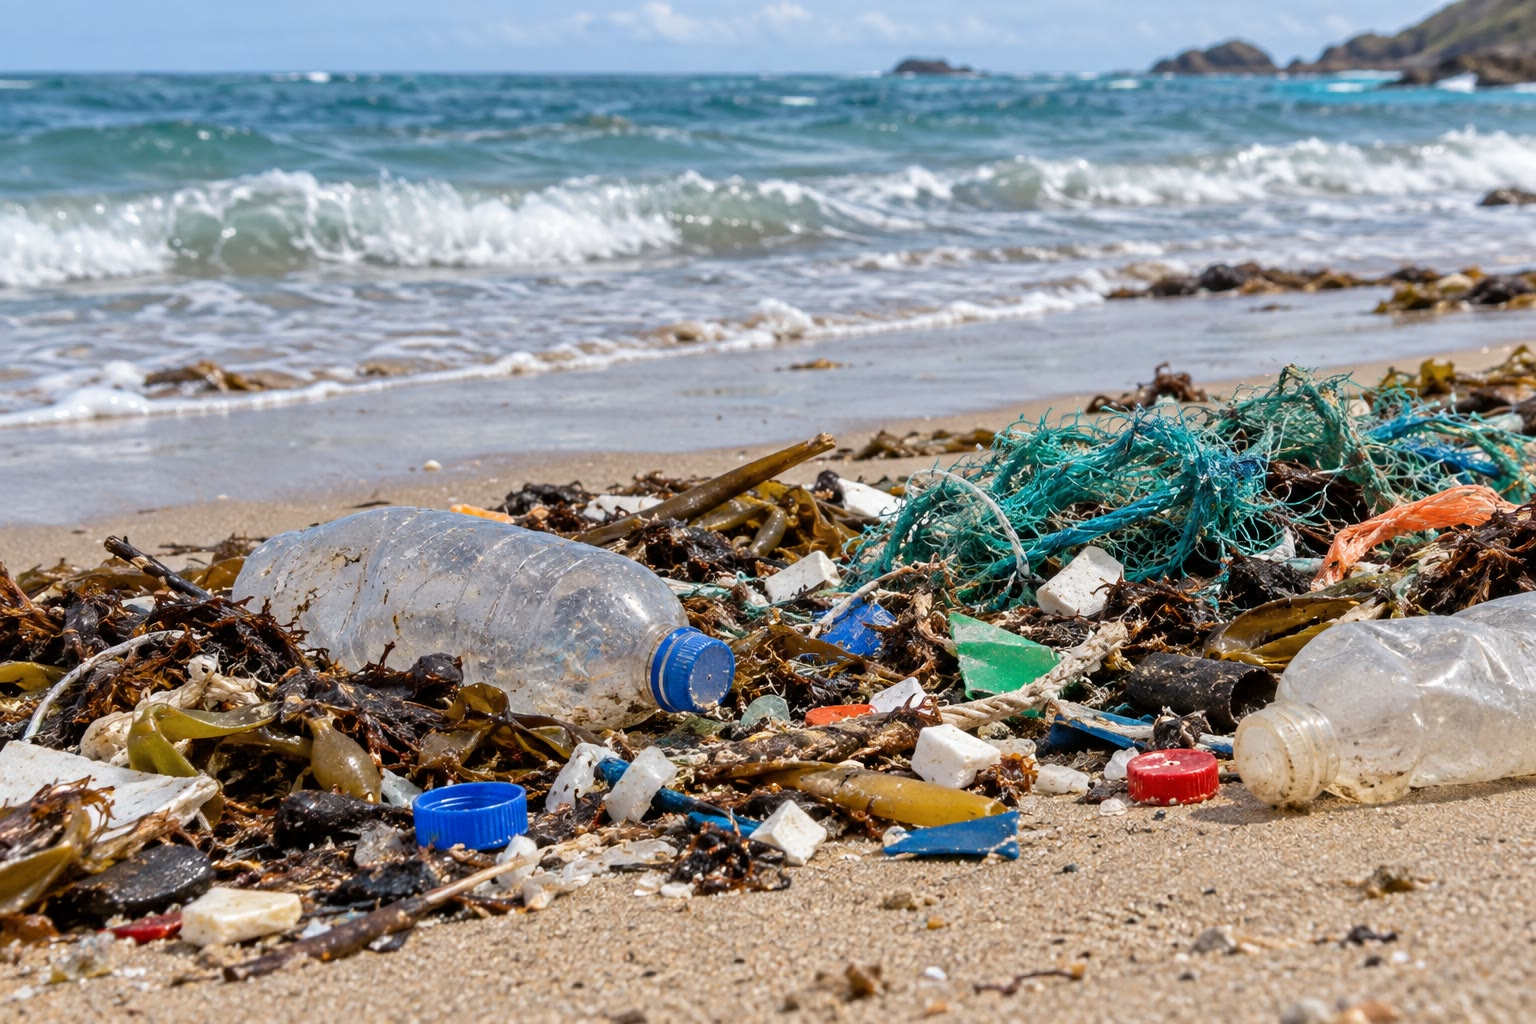
\includegraphics[width=\linewidth,height=4.6cm,keepaspectratio]{images/book1/ai/g8-beach-litter.jpg}

{\small Aangespoeld plastic afval op een strand.}
\end{minipage}\hfill
\begin{minipage}[t]{0.48\linewidth}\centering
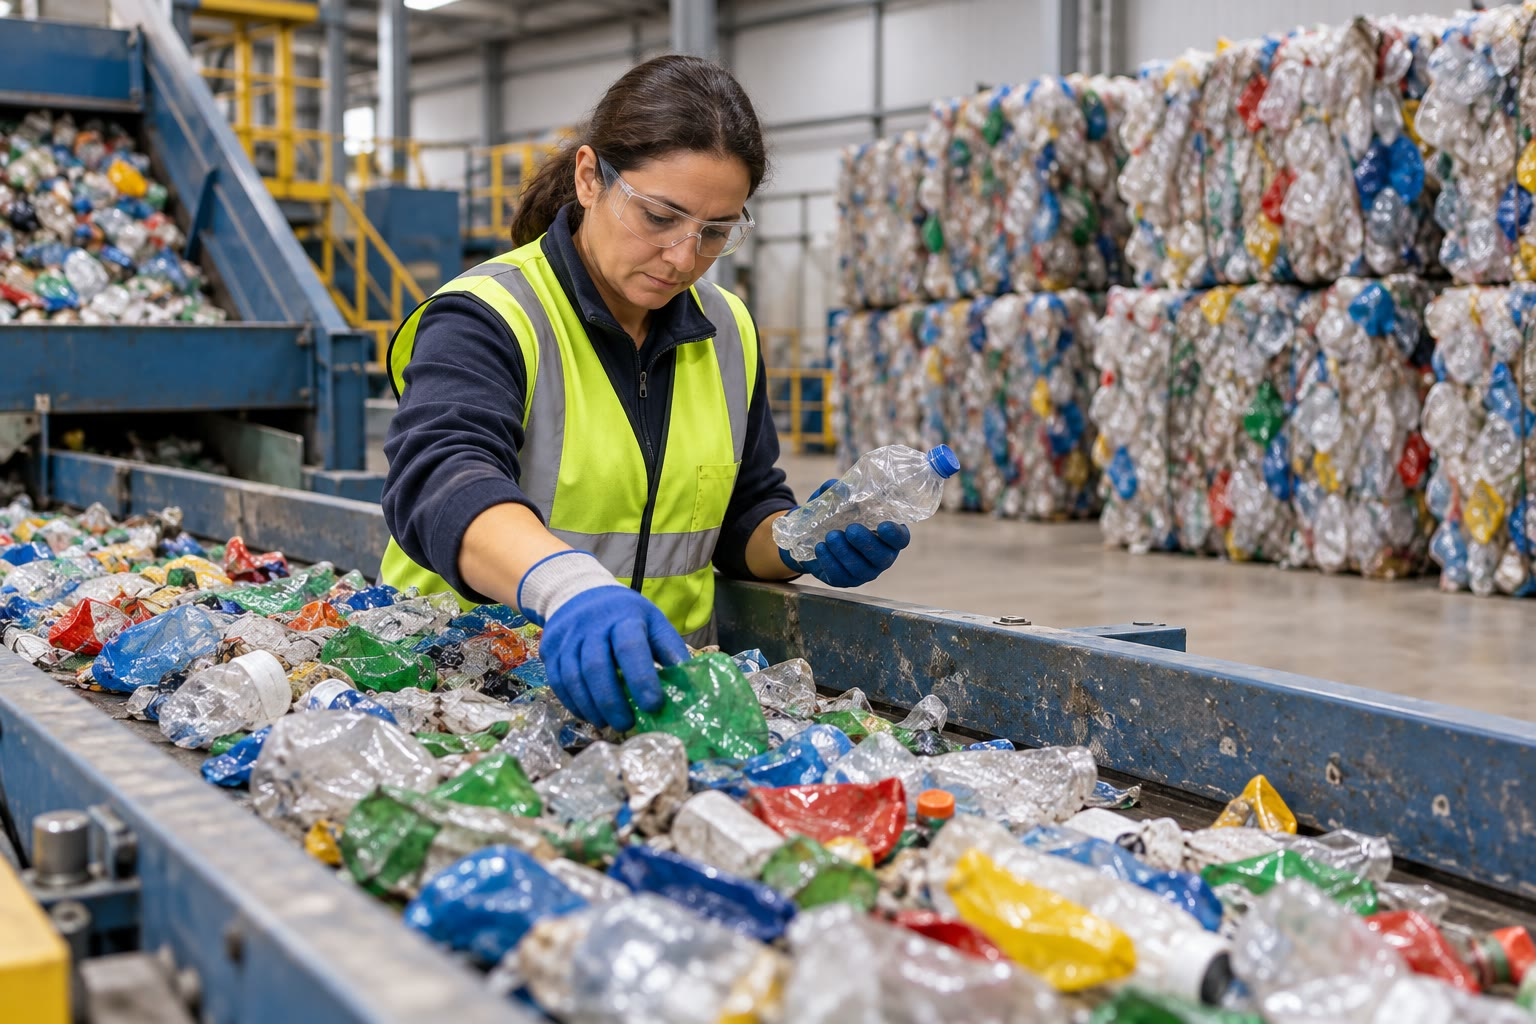
\includegraphics[width=\linewidth,height=4.6cm,keepaspectratio]{images/book1/ai/g8-sorting-line.jpg}

{\small Een sorteerband in een recyclingbedrijf voor \omterm{def:g8:plastics:plastic}{kunststoffen}.}
\end{minipage}
\end{omfigure}

\begin{remark}[Kunststoffen verbranden]\label{rem:g8:plastics:burning}
\omterm{def:g8:plastics:plastic}{Kunststoffen} \omterm{def:g4:what-a-fire-needs:burning}{branden}, en bij een \omterm{def:g8:combustion-and-fuels:complete}{volledige verbranding} geven ze
koolstofdioxide. Maar in een tuinvuur \omterm{def:g4:what-a-fire-needs:burning}{verbranden} ze onvolledig en komen
er roet, koolstofmono-oxide en andere schadelijke stoffen vrij; PVC, dat
chloor bevat, geeft waterstofchloride af, een bijtend gas.
Kunststofafval wordt alleen verbrand in verbrandingsovens die gebouwd
zijn om hun rookgassen te reinigen.
\end{remark}

\section{Oefeningen}

\begin{exercise}[$\star$]\label{exo:g8:plastics:1}
Natuurlijk, kunstmatig of synthetisch? Katoen, nylon, papier, wol,
polystyreen, viscose.
\end{exercise}

\begin{exercise}[$\star$]\label{exo:g8:plastics:2}
Van welke \omterm{def:g5:raw-materials-and-recycling:raw-material}{grondstof} worden de meeste \omterm{def:g8:plastics:plastic}{kunststoffen} gemaakt?
\end{exercise}

\begin{exercise}[$\star$]\label{exo:g8:plastics:3}
Welke \omterm{def:g8:plastics:plastic}{kunststof} heeft code 1? Noem een voorwerp dat ervan gemaakt is.
\end{exercise}

\begin{exercise}[$\star$]\label{exo:g8:plastics:4}
Wat is het verschil tussen een \omterm{def:g8:plastics:thermoplastic}{thermoplast} en een \omterm{def:g8:plastics:thermoplastic}{thermoharder}?
\end{exercise}

\begin{exercise}[$\star\star$]\label{exo:g8:plastics:5}
Op een yoghurtbeker staat code 5. Noem de \omterm{def:g8:plastics:plastic}{kunststof}, en zeg of je die in
principe kunt smelten en opnieuw vormen.
\end{exercise}

\begin{exercise}[$\star\star$]\label{exo:g8:plastics:6}
Waarom betekent een driehoek van pijlen op een voorwerp niet dat het
voorwerp gerecycled zal worden?
\end{exercise}

\begin{exercise}[$\star\star$]\label{exo:g8:plastics:7}
Waarom is het handvat van een koekenpan vaak van een \omterm{def:g8:plastics:thermoplastic}{thermoharder}
gemaakt en niet van een \omterm{def:g8:plastics:thermoplastic}{thermoplast}?
\end{exercise}

\begin{exercise}[$\star\star$]\label{exo:g8:plastics:8}
Welk percentage van de gebruikte \omterm{def:g8:plastics:plastic}{kunststof} werd volgens de getallen van
dit hoofdstuk in 2019 afval? Rond af op een geheel getal.
\end{exercise}

\begin{exercise}[$\star\star$]\label{exo:g8:plastics:9}
Waarom mag PVC nooit in een tuinvuur verbrand worden?
\end{exercise}

\begin{exercise}[$\star\star$]\label{exo:g8:plastics:10}
Een school gebruikt per week 300 flessen van elk \qty{25}{g}, gedurende
36 weken per jaar. Hoeveel \omterm{def:g8:plastics:plastic}{kunststof} is dat in een jaar?
\end{exercise}

\begin{exercise}[$\star\star\star$]\label{exo:g8:plastics:11}
Polyetheen bestaat alleen uit koolstof en waterstof. Noem de
\omterm{def:g7:chemical-reactions:reactant}{reactieproducten} van zijn \omterm{def:g8:combustion-and-fuels:complete}{volledige verbranding}. Leg uit waarom het
\omterm{def:g4:what-a-fire-needs:burning}{verbranden} ervan koolstofdioxide aan de \omterm{def:g4:air-a-mixture-of-gases:air}{lucht} toevoegt, net als een
\omterm{def:g8:combustion-and-fuels:fossil}{fossiele brandstof}.
\end{exercise}

\begin{exercise}[$\star\star\star$]\label{exo:g8:plastics:12}
Leg uit hoe een plastic fles die op zee verloren is gegaan, jaren later
als microplastic in een vis terecht kan komen.
\end{exercise}

\section{Probleem: De sorteerband}

\begin{problem}[{Weekendprobleem --- een ton gebruikte flessen, hun codes,
en de schone kunststofvlokken die uit de fabriek komen}]
\label{pb:g8:plastics:1}
Een recyclingbedrijf ontvangt balen gebruikte drankflessen. Een typische
baal van \qty{1}{t} (\qty{1000}{kg}) bevat, in massa: \qty{80}{\percent}
flessen van PET, \qty{12}{\percent} doppen (HDPE en PP),
\qty{5}{\percent} etiketten (PP-folie) en \qty{3}{\percent} vuil en
restjes vloeistof. Machines scheiden de doppen en etiketten van de
flessen, het PET wordt tot vlokken gemalen en de vlokken worden gewassen;
bij het wassen gaat \qty{2.5}{\percent} van het PET verloren. De schone
vlokken worden gesmolten en tot de vezels van fleecejacks gesponnen.

\medskip
\noindent\textbf{Deel I --- De \omterm{def:g8:plastics:plastic}{kunststoffen}.}
\begin{enumerate}
  \item Welke code staat er op de flessen? En op de doppen?
  \item Zijn deze \omterm{def:g8:plastics:plastic}{kunststoffen} natuurlijk, kunstmatig of synthetisch?
  \item Kun je PET opnieuw smelten en spinnen? Wat voor \omterm{def:g8:plastics:plastic}{kunststof} is het
        dus?
  \item Waarom worden de doppen en etiketten van de flessen gescheiden
        voordat het PET gesmolten wordt?
\end{enumerate}

\medskip
\noindent\textbf{Deel II --- De baal.}
\begin{enumerate}[resume]
  \item Hoeveel PET bevat een baal?
  \item Hoeveel doppen? Hoeveel etiketten?
  \item Welke massa van de baal is geen \omterm{def:g8:plastics:plastic}{kunststof}?
  \item Welk percentage van de baal is \omterm{def:g8:plastics:plastic}{kunststof}?
\end{enumerate}

\medskip
\noindent\textbf{Deel III --- De vlokken.}
\begin{enumerate}[resume]
  \item Hoeveel PET gaat er bij het wassen verloren?
  \item Voor een fleecejack is \qty{0.39}{kg} PET-vezel nodig. Waarom is
        het beter om het van vlokken te maken dan van nieuw PET?
  \item Het bedrijf zou de doppen en etiketten kunnen \omterm{def:g4:what-a-fire-needs:burning}{verbranden} voor
        warmte in plaats van ze te recyclen. Noem het gas dat dit aan de
        \omterm{def:g4:air-a-mixture-of-gases:air}{lucht} zou toevoegen.
  \item Bereken de massa schone PET-vlokken die één baal oplevert.
\end{enumerate}
\end{problem}
